\documentclass[tikz]{standalone}

\usepackage{tikz}
\usetikzlibrary{shapes.geometric, arrows}


\tikzstyle{start} = [minimum height=1cm]
\tikzstyle{box} = [rectangle, minimum width=1.25cm ,text width=1.9cm,minimum height=1.7cm,text centered, draw=black]
\tikzstyle{fgain} = [isosceles triangle,isosceles triangle apex angle=60,draw=black]
\tikzstyle{fbox} = [rectangle, minimum width=0.75cm,minimum height=0.75cm,text centered, draw=black]
\tikzstyle{foperation} = [circle, radius=0.2, minimum size=0.75cm,inner sep=0pt, draw=black]
\tikzstyle{stop} = [minimum height=1cm]

\begin{document}
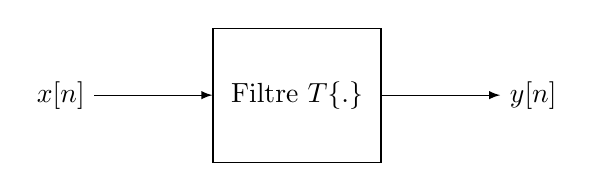
\begin{tikzpicture}[node distance=3cm]
    \node[start] (start) {$x[n]$};
    \node[box,right of=start] (filter) { Filtre $T\{.\}$};
    \node[stop,right of=filter] (end) {$y[n]$};
    \draw[->,>=latex] (start) -- (filter);
    \draw[->,>=latex] (filter) -- (end);
\end{tikzpicture}
\end{document}